\documentclass{acmsmall}
\usepackage[ruled]{algorithm2e}
\renewcommand{\algorithmcfname}{ALGORITHM}
\SetAlFnt{\small}
\SetAlCapFnt{\small}
\SetAlCapNameFnt{\small}
\SetAlCapHSkip{0pt}
\IncMargin{-\parindent}

\makeatletter
\def\ps@headings{%
\def\@oddhead{\mbox{}\scriptsize\rightmark\hfil\thepage}%
\def\@evenhead{\scriptsize\thepage\hfil\leftmark\mbox{}}%
\def\@oddfoot{}%
\def\@evenfoot{}}
\makeatother
\usepackage{caption}
\pagestyle{headings}
\usepackage{cite}
\usepackage{rotating}
\usepackage{amssymb,amsmath}
\usepackage{multirow}
\usepackage{verbatim}
\addtolength{\textfloatsep}{-5mm} \addtolength{\floatsep}{-3mm}
\usepackage{lettrine}
\usepackage{flushend}
\usepackage{array,booktabs,arydshln,xcolor}
\usepackage{graphicx}
\newcommand\VRule[1][\arrayrulewidth]{\vrule width #1}

\def\draftmode{}
\ifx\draftmode\undefined
\newcommand{\mcomment}[1]{}
\else
\newcommand{\mcomment}[1]{$\Longleftarrow${\bf $<$#1$>$} }
\fi

\DeclareGraphicsExtensions{.eps,.png}


\begin{document}

\markboth{}{Hiding Data in HTTP: A Network Steganography Project}

\title{Hiding Data in HTTP: A Network Steganography Project}
\author{Sean Donovan, Sathyanarayanan Gunasekaran, Sarthak Grover, Karim Habak, and Ben Jones}
\maketitle

\section{Abstract}
To prevent a censor from being able to trivially recognize a Tor data stream, the Pluggable Transport framework was established to allow developers to mask Tor data by masquerading as something innocuous. 

HyperText Pluggable Transport (HTPT) is a SOCKS proxy that is designed to be the precursor of a Tor Pluggable Transport. HTPT is designed to mask a data stream by converting the data stream into a series of HTTP requests, responses, and image data. It is extensible in that further encoding schemes can be used to encode stream data into HTTP-related resources. For instance, a developer could create a new encoding for Scalable Vector Graphics (SVG) to hide data within the XML elements of the filetype. HTPT provides resistance to Deep Packet Inspection (DPI) by appearing to be an HTTP stream, which are generally not blocked by even the most repressive of governments, due to the innocuous nature of the majority of HTTP traffic. 

\section{Introduction}
Internet censorship is a fact of life in many locations and circumvention tools are the only access some citizens have to unfiltered information. The censor restricts access to these circumvention utilities to maintain information control and a cat and mouse game is born as the circumvention tools try to evade detection. Tor is a useful tool for circumventing Internet censorship that encrypts data and provides an untraceable method for accessing data. 

Unfortunately, Tor is detectable. The stream is fingerprintable. Tor developers came up with the Pluggable Transport framework\cite{Ref1}.
 %The initial goal of the project was to develop a Pluggable Transport\cite{Ref1}, but this was found to be not feasible in the timeframe of the project.
%A Pluggable Transport is an obfuscation layer between a Tor client and a Tor bridge to prevent detection of otherwise  well known Tor data streams. 
Pluggable Transports consist of two parts: a client and a server. Typically these are slightly different obfuscate/de-obfuscate layers, however they can be very different depending on what the obfuscation mechanism is. This obfuscate/de-obfuscate layers operates below Tor and relays Tor traffic in a form that is difficult for DPI device to detect in a computationally cost effective manner. In some cases, the Pluggable Transport mechanism mimics or tunnels through an existing protocol\cite{Ref2,Ref3} and in other cases, the transport mechanism tries to appear random\cite{Ref4}. Implementing the obfuscate/de-obfuscate layers as a SOCKS proxy is a proof of concept, and allows for further development into a proper Pluggable Transport

Based on this, we decided that making a obfuscation layer that can be used by Tor along with many other application. We have developed a socket proxy that sits below user applications to provide a level of obfuscation such that the data stream is not an trivially detected as the original stream. 

For our proxy, the obfuscation layer will hide data within HTTP resources in HTTP requests and responses. More specifically, data will be encoded to look like images or more general HTTP traffic and either uploaded to the server or downloaded to the client. By allowing for both upload and download, we are not limiting the application of this pluggable transport to primarily unidirectional traffic. %This can be used by not \emph{just} Tor, but also by web browsers and any other SOCKS client.

\section{Design}
HTPT is designed to be a SOCKS proxy. Since client and server HTTP traffic is different, the encoding in each direction is asymmetric. That is, the client- and server-side encoding is different, and the decoding is similarly asymmetric such that the client can decode server data and vice versa. Below the threat model will be discussed, followed by a discussion of the goals, with HTPT's architecture following, then describing implemented encoding schemes.

\subsection{Threat Model}
The threat model that HTPT is designed to counter includes the following:
\begin{enumerate}
  \item Lightweight DPI is used. This includes looking at headers and parts of the packets transiting the DPI device block entire flows, but does it does not include reassembly of streams or other stateful information.
  \item Stateful DPI is not used frequently. This is due to the cost of remembering state information about a particular connection or series of connections.
  \item HTTP traffic is not widely blocked. Specific sites may be blocked but through an alternate mechanism (e.g., DNS redirection).
  \item Connection to a generic web server for a long period of time may be considered unusual, but connecting to an image server for a long period of time is less unusual.
  \item Image files transferred over HTTP can be verified to be valid images. Manual checking of image data will not happen due to cost.
\end{enumerate}

\subsection{Design Goals}
With the threat model in mind, the main goal is to make it more costly for a censor to discover the underlying Tor stream. To do this an image gallery website that hides a Tor bridge was chosen as a very high level design. Authenticated users will be allowed to send Tor traffic to the web server, while non-authenticated users will be returned a simple image gallery website. This means that the website must be able to correctly identify Tor and non-Tor traffic, and direct the traffic to the correct handlers. 

An additional goal is to provide plausible traffic going from the client to the server and vice versa. This effectively means that multiple encoding schemes must be created, as client traffic looks significantly different from server traffic in HTTP. 

Allow for users to upload significant amounts of data is also a goal. Most usage of HTTP sees the server sending significantly more data to the client than the client to the server, it is realistic in the case of an image gallery website for the user to upload significant amounts of data in the form of new images.

Preventing obvious fingerprintable behaviors is also a desired goal. This means that the server should not always send 128KB JPEGs, but rather it should vary the size and data type regularly.  

Reasonable performance, as measured by both `goodput' and latency, is a desired goal. Latency is most important for users of interactive websites, while reasonable goodput is required for uploading and downloading bulk data. 

\subsection{Motivations}
The main motivations for adding yet another layer to an already tall stack is similar to how IPSEC is meant to work. This seems like it would be excessive overhead, but is primarily to hide a layer (Tor, in this case) that is providing security that should not be found. It is a proper layer that can be removed or inserted as necessary, and is not actually required to exist. 

\cite{Ref2} discusses the need to use the applications themselves and not just the protocol to obfuscate traffic. Otherwise adversaries can easily identify obfuscated traffic by finding differences in implementations of the protocols by the application and by the obfuscating layer. For example, Apache may implement a particular part of HTTP different from specification, while the obfuscating layer may not. This would make it susceptible to fingerprinting. As such, using actual applications for generating HTTP requests and responses will be necessary.

\subsection{Architecture}
The overall architecture is represented in Figure~\ref{fig:overall_arch}. It is a basic client-server model, but with several important additional layers.

\begin{figure}[t]
\centering
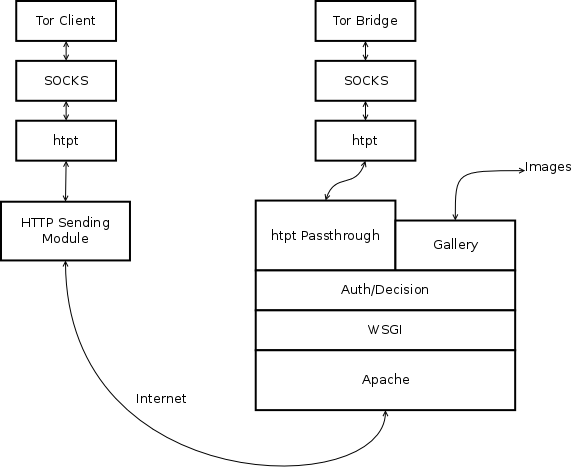
\includegraphics[width=0.7\textwidth]{Overall_architecture}
\caption{Overall Architecture}
\label{fig:overall_arch}
\end{figure}

On the client-side, there is a SOCKS interface that HTPT presents to its user, typically Tor as is represented here. HTPT is then connected to an HTTP sending module that interacts with the server-side.

The server-side from the top down is very similar: Tor connects via SOCKS with HTPT. At this point, the design diverges significantly. For this, looking from the bottom up is useful. 
The client uses Selenium, a web browser orchestration framework, in conjunction with the Tor Browser Bundle, a packaged Tor client and Firefox web browser, to properly simulate web traffic and handle errors. 
The client connects to Apache, which is running the Web Server Gateway Interface module. This is a specification to allow web servers to communicate with web applications \cite{Ref16}. This is used to interface with the Authorization/Decision module that is part of the HTPT package. It is used to decide whether to send the traffic to the Image Gallery (for non-authorized traffic), or to the HTPT Passthrough (for authorized traffic). This is what it sounds: a simple passthrough. Traffic is then handed off the HTPT. 

The reverse is also true: traffic from the Tor Bridge to the Tor client goes through the same layers, just in reverse. 

\begin{figure}[b]
\centering
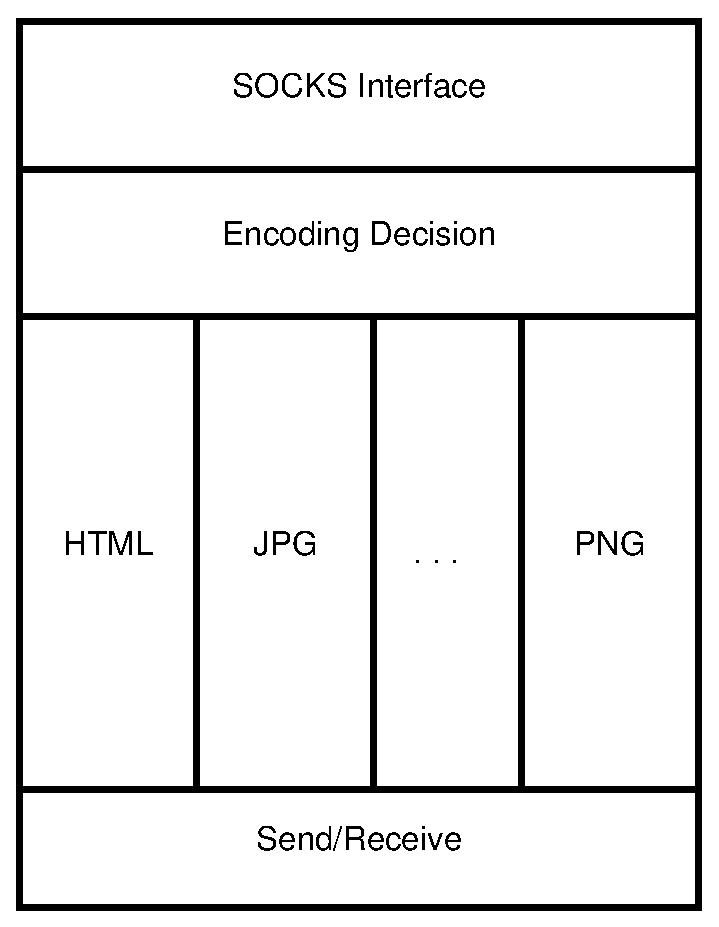
\includegraphics[width=0.3\textwidth]{htpt_architecture}
\caption{Modules within HTPT}
\label{fig:htpt_modules}
\end{figure}

Within HTPT, there are four main modules, as can be seen in Figure~\ref{fig:htpt_modules}. The SOCKS interface is the primary interface for communicating with Tor. This can also be used for other clients in a similar fashion, but in a much more limited manner.

The Encoding Decision module is the main location where anti-fingerprinting measures are taken. This module varies the encoding scheme and encoding amount such that the same style of data is not seen consistently. This is done by using a timer to buffer data up to a random amount of data to be sent. If that random amount is seen before the timer expires, it is sent, and a new random time and amount of data is chosen. This should make inter-arrival times more random than Tor normally is. 

Which encoding scheme is chosen depends on whether HTPT is acting in the client or server mode, and the data rate. This is measured based on the pervious transmission. That is, if 1000 bytes was received in the previous 10 milliseconds, the data rate can be calculated as being 100,000 bytes per second. This assumes that the data rate stays constant, which is why the time and buffer sizes are used in conjunction with each other.

This also acts as a framing module. Since each send operation opens a transient connection, reordering of data is vital. To handle this, sequence numbers are assigned by the Encoding Decision module. It is responsible for reorder of received data, for similar reasons. 

The Send/Receive module is an interface module. It is different for both the client and the server, as the lower interface is different. The client-side Send/Receive module will interface with an HTTP Sending Module, while the server-side will interface with the HTPT Passthrough.

Between the Send/Receive module and the Encoding Decision module lies the encoding modules themselves. They have a standard interface and are designed in such a way that new encoding modules can be added. For instance, if a developer wanted to create CSS encoder that generated CSS that encodes data, it could be added to the existing encoders.

Of note: this is a pull protocol. The client can push data to the server, but the server must be polled for more data. This is due to the nature of HTTP, and such mechanisms for polling for more data already exist: see how AJAX systems work.

\subsection{Encoding Schemes}
There are currently six developed encoding modules. Each takes in a common header, optionally appends its own header, and a quantity of data. This is then encoded and sent out. The header is retrieved from the Encoding Decision module, such that consistent sequence numbers can be retrieved. Local headers can consist of padding information, if the particular item sends fixed-width data chunks. 

\begin{enumerate}
  \item \emph{Advertising URL Encoder} --- This encodes 40 bytes of data at a time by mimicking an advertising header. These frequently have 80-character hex-encoded identifiers contained within them, and are useful for encoding small amounts of data from the client to the server.
  \item \emph{Google Search String Encoder} --- This encodes variable amounts of data, albeit small amounts of data. Initial implementation uses 16 common English words to represent 4-bits of data, effectively acting as a hex encoder. These are then places in what looks like a Google search string that can be decoded on the receiving end.
  \item \emph{Baidu Search String Encoder} --- This is a similar scheme as the Google Search String Encoder, except that it is designed to create Baidu-like search strings.
  \item \emph{BMP Encoder} --- This is the most basic image encoder. A valid bitmap header is created, then the raw data makes up the image data.
  \item \emph{JPEG Encoder} --- By using lossless JPEGs, data can be sent across without loss. This uses the BMP Encoder, and converts it into a lossless JPEG to be sent by either the client or server.
  \item \emph{PNG Encoder} --- This is a similar scheme as the JPEG Encoder, with PNGs as output.
\end{enumerate}

\subsection{Framing and Performance Implications}
As noted above, the encoding is an encapsulation scheme. The data from Tor, or any other SOCKS enabled client, is treated as a byte-stream, much like data that is sent via TCP. A 4-byte header is attached on each segment sent. The segment is then wrapped based on the encoding scheme, which is where the overhead comes into play.


TODO: NEED A DIAGRAM OF HEADER


As one of the design goals is to have reasonable goodput performance, the overhead must be discussed. 


TODO: NEED A TABLE OF OVERHEAD RATIOS, MINIMUM AND MAXIMUM, number of bytes of overhead per item.

\section{Testing}

Testing is an ongoing process. During development unit tests are used, and after development, performance tests are used. 

\subsection{Unit Tests}
Each individual module is being tested during development. These tests are tailored to the type of module being tested

For instance, each encoding module is connected to itself to verify the what is encoded can be decoded correctly, without loss. This prevents accidental corruption of data by the encoding modules, which would cause the Tor connection to be taken down.

Integration tests between modules also occur, to verify proper functionality. For instance, testing of the image gallery application along with Apache is necessary independent of HTPT development. 

\subsection{Performance Characterization}
As one of the goals is reasonable performance, various performance assesments are necessary. Since the goal was about relative performance, three iterations for each test is used: one with just a browser, one with the browser and Tor, and one with the browser, Tor, and HTPT. This will give relative performance for comparison. 

The following test configurations are being used for performance characterizations:  
\begin{enumerate}
  \item Loading twenty popular web pages --- This will be a demonstration of latency. By finding the total time it takes to perform this operation, additional latency can be seen. This test will not work directly with the browser and HTPT, so it is not being performed directly. 
  \item Downloading 1 gigabyte file over HTTP --- This is an example of a bulk download that will allow measurement of goodput.
  \item Uploading 1 gigabyte file over HTTP --- Since this is an assymetric encoding scheme, upload goodput testing is required.
\end{enumerate}

%\subsection{DPI Testing}
%In an ideal world, where there is unlimited testing time, the testing framework developed by Tor \cite{Ref14} would be used. 
\section{Progress}

%%%
% What is done
% What is left to do
% Mention descaling due to overly optimistic assumptions - Python bindings for Headless webkit had been phased out
%%%

\section{Future Work}

There are significant possibilities for expanding this work. 
%The initial intent was to develop a Pluggable Transport, and this is the most important piece of future enhancement. This would involve either modifying obfsproxy or manually integrating with with Tor.

The biggest improvement could be made in the framing module.  This module could vary the encoding scheme and encoding amount such that the same style of data is not seen consistently. This can be done by using a timer to buffer data up to a random amount of data to be sent. If that random amount is seen before the timer expires, it is sent, and a new random time and amount of data is chosen. This should make inter-arrival times more random than Tor normally is. 

Which encoding scheme is chosen depends on whether HTPT is acting in the client or server mode, and the data rate. This is measured based on the pervious transmission. That is, if 1000 bytes was received in the previous 10 milliseconds, the data rate can be calculated as being 100,000 bytes per second. This assumes that the data rate stays constant, which is why the time and buffer sizes are used in conjunction with each other.

Integrating this into the obfsproxy framework and bundling with the Tor Browser Bundle would be good to do in the future.

Another further enhancement is to enhance authentication. Current authentication is basic HTTP's basic access authentication. This is very simplistic, and any information is sent in plaintext. Clearly, that is a security problem, so a more secure authentication scheme is justified.

Replay attacks need to be looked at in greater detail to determine if further mitigation is needed.

%There is the possibility of the fingerprinting the header that all packets have. It would be hard to do, and would require stateful DPI. To mitigate this, encrypting the header or the entire packet again would be mitigate this. Encrypting the header is less costly computationally, and would be more than sufficient. Implementing some sort of key exchange algorithm (e.g., Diffie-Hellman) would be necessary as well.

\nocite{Ref1,Ref2,Ref3,Ref4,Ref5,Ref6,Ref7,Ref8,Ref9,Ref10,Ref12,Ref13,Ref14,Ref15 }

\bibliographystyle{ACM-Reference-Format-Journals}
\bibliography{Tor}
\end{document}